\documentclass[12pt,a4paper]{article}
\usepackage[utf8]{inputenc}
\usepackage[T1]{fontenc}
\usepackage[french]{babel}
\usepackage{amsmath, amssymb}
\usepackage{graphicx}
\usepackage{geometry}
\geometry{margin=2cm}
\usepackage{enumitem}
\usepackage{float}
\usepackage{fancyhdr}
\usepackage{titlesec}
\usepackage{amsmath}
\pagestyle{fancy}

% Nettoyer les styles par défaut
\fancyhf{}

% En-têtes
\fancyhead[L]{Fiches d'exercices pour Maximilien (8)} % à gauche
\fancyhead[R]{Matteo Dubresson} % à droite

% Pieds de page
\fancyfoot[C]{\thepage} % numéro de page centré

%Titre et généralités
\title{Fiche d'exercices \\ pour Maximilien (8)}
\date{28/10/2026}
\author{}

%Espace entre les subsections
\titlespacing*{\subsection}{0pt}{5ex plus 0.5ex minus 0.2ex}{1.5ex plus 0.2ex}




\begin{document}

\maketitle


\subsection*{Exercice 1 : (metropole 1 2026)}
Lorsque la pièce atteint la température de $20\text{ \textdegree{}C}$, le système de chauffage s'éteint et la pièce refroidit.

On modélise la température de la pièce par la suite $(u_n)$ définie par $u_0 = 20$ et pour tout entier naturel $n$ :
$$u_{n+1} = 0,965u_n + 0,35 + 0,07\text{e}^{-0,1n}$$
où $n$ est un nombre entier exprimant le temps écoulé en dizaines de minutes.

\begin{enumerate}
    \item Montrer que $u_1 = 19,72$.
    \item Montrer par récurrence que, pour tout entier naturel $n$, on a $u_n > 10$.
\end{enumerate}

On admet que la suite $(u_n)$ est décroissante.

\begin{enumerate}
    \setcounter{enumi}{2}
    \item En déduire que la suite $(u_n)$ est convergente.
    \item On note $\ell$ la limite de la suite $(u_n)$.
    \begin{enumerate}
        \item Justifier que cette limite est solution de l'équation $x = 0,965x + 0,35$.
        \item Déterminer $\ell$ et interpréter le résultat dans le contexte de l'exercice.
    \end{enumerate}
    \item On rappelle que le système de chauffage se met en marche automatiquement dès que la température de la pièce est inférieure ou égale à $18\text{ \textdegree{}C}$.
    \begin{enumerate}
        \item Recopier et compléter les lignes 4, 5 et 6 du programme écrit en langage Python ci-dessous, afin qu'il renvoie le nombre de dizaines de minutes à partir duquel le système de chauffage se remettra en marche.
        
        \begin{center}
        \begin{tabular}{|l l|}
            \hline
            1. & \texttt{def marche() :} \\
            2. & \quad \texttt{n = 0} \\
            3. & \quad \texttt{u = 20} \\
            4. & \quad \texttt{while ... :} \\
            5. & \quad \quad \texttt{u = ...} \\
            6. & \quad \quad \texttt{n = ...} \\
            7. & \quad \texttt{return n} \\
            \hline
        \end{tabular}
        \end{center}
        
        \item Déterminer le temps, en dizaines de minutes, à partir duquel le système de chauffage se remettra en marche.
    \end{enumerate}
\end{enumerate}

\subsection*{Exercice 2 : (metropole 1 2026)}
On considère la fonction $f$ définie sur l'intervalle $]-1 ; +\infty[$ par :
$$f(x) = a + \frac{b\ln(x+1)}{x+1}$$
où $a$ et $b$ sont des réels, et $\ln$ désigne la fonction logarithme népérien.

On admet que la fonction $f$ est deux fois dérivable sur $]-1 ; +\infty[$. On note $f'$ sa fonction dérivée et $f''$ sa fonction dérivée seconde.

\begin{center}
\textbf{Partie A}
\end{center}

L'objectif de cette partie est de déterminer les valeurs de $a$ et $b$ de sorte que la courbe représentative de la fonction $f$ sur $[0 ; +\infty[$ corresponde à celle tracée dans le repère orthonormé ci-dessous :

\begin{figure}[H]
    \centering
    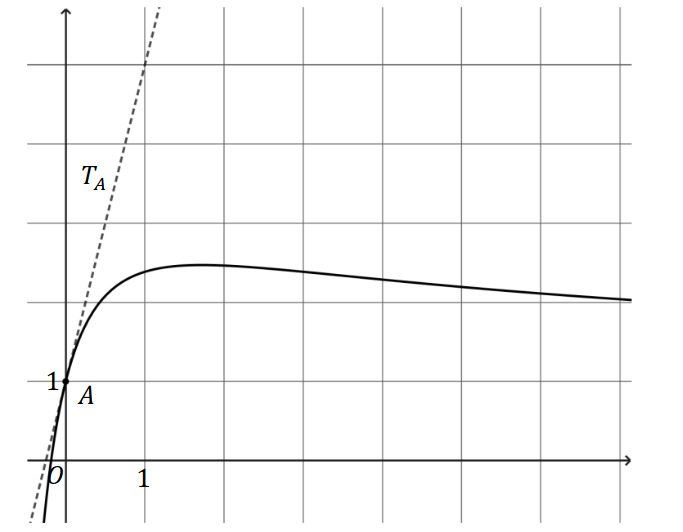
\includegraphics[width=0.6\textwidth]{courbe_f.png}
    \caption{Représentation graphique de la fonction $f$.}
\end{figure}

On précise que la droite $T_A$ est la tangente à la courbe représentative de la fonction $f$ au point $A(0 ; 1)$.

\begin{enumerate}
    \item Justifier que $a = 1$.
    \item En utilisant le graphique :
    \begin{enumerate}
        \item Donner la valeur de $f'(0)$. Justifier.
        \item Donner le signe de $f''(1)$. Justifier.
    \end{enumerate}
    \item 
    \begin{enumerate}
        \item Montrer que pour tout réel $x$ appartenant à $]-1 ; +\infty[$, on a :
        $$f'(x) = \frac{b(1 - \ln(x+1))}{(x+1)^2}$$
        \item En déduire la valeur de $b$.
    \end{enumerate}
\end{enumerate}

\newpage

\begin{center}
\textbf{Partie B}
\end{center}

On admet dans la suite de l'exercice que la fonction $f$ est définie sur $]-1 ; +\infty[$ par :
$$f(x) = 1 + \frac{4\ln(x+1)}{x+1}$$

\begin{enumerate}
    \item Justifier que la droite d'équation $y = 1$ est asymptote à la courbe représentative de la fonction $f$.
    \item Résoudre l'inéquation $1 - \ln(x+1) > 0$ sur $]-1 ; +\infty[$.
    \item On admet que $\lim_{x \to -1} f(x) = -\infty$.

    Dresser le tableau de variation complet de la fonction $f$ en indiquant la valeur exacte de son extremum. Justifier.
    \item Montrer que l'équation $f(x) = 1,5$ admet une unique solution dans l'intervalle $[2 ; +\infty[$. En donner une valeur arrondie à $10^{-1}$.
\end{enumerate}



\subsection*{Exercice 3 : (metropole 2 2026)}

\begin{center}
\textbf{Partie A}
\end{center}

Soit $f$ une fonction définie et dérivable sur l'intervalle $[0 ; +\infty[$ dont on donne ci-dessous une partie de la courbe représentative $\mathcal{C}_f$ dans un repère orthogonal. On note $f'$ sa fonction dérivée.


\begin{figure}[H]
    \centering
    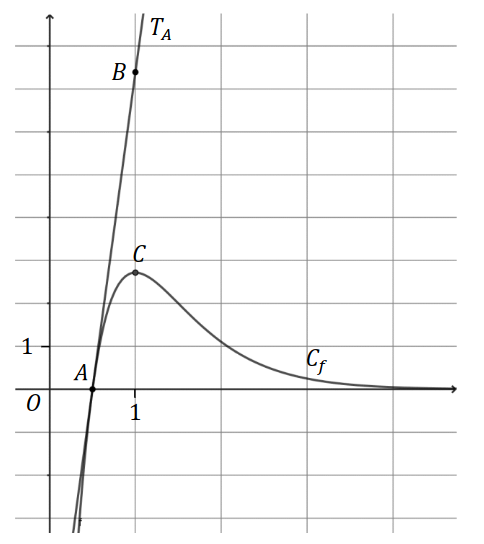
\includegraphics[width=0.4\textwidth]{image_1_exo4.png}
\end{figure}



On précise que :
\begin{itemize}
    \item la courbe $\mathcal{C}_f$ admet une tangente parallèle à l'axe des abscisses au point $C$ d'abscisse $1$ ;
    \item la tangente $T_A$ à la courbe $\mathcal{C}_f$ au point $A\left(\frac{1}{2} ; 0\right)$ passe par le point $B(1 ; \text{e}^2)$.
\end{itemize}

\begin{enumerate}
    \item À l'aide du graphique ci-contre :
    \begin{enumerate}
        \item[a.] Donner $f'(1)$.
        \item[b.] Donner la solution de l'équation $f(x) = 0$ sur l'intervalle $[0 ; 3]$.
    \end{enumerate}
    \item Déterminer $f'\left(\frac{1}{2}\right)$.
    \item Parmi les trois courbes $\mathcal{C}_1$, $\mathcal{C}_2$ et $\mathcal{C}_3$ ci-dessous, deux représentent des primitives de la fonction $f$. Indiquer lesquelles et justifier.
\end{enumerate}



\begin{figure}[H]
    \centering
    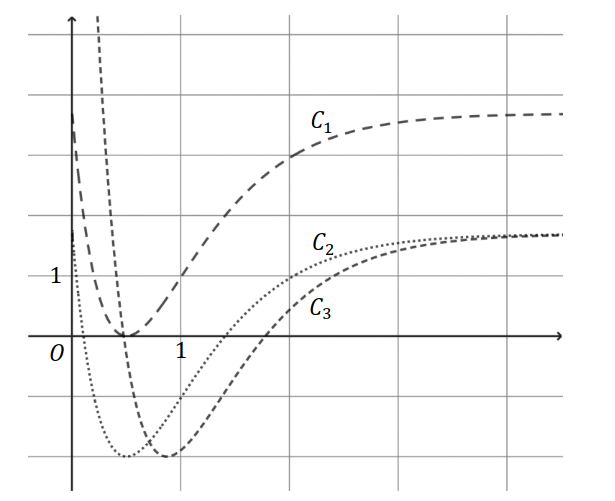
\includegraphics[width=0.5\textwidth]{image_2_exo4.png}
\end{figure}

\begin{center}
\textbf{Partie B}
\end{center}

Un industriel doit créer un logo représentant la forme ci-contre (Fig. 1). La dimension de $0,3\text{ cm}$ indiquée sur la figure est une contrainte imposée par le client.


\begin{figure}[H]
    \centering
    \begin{minipage}[c]{0.35\textwidth}
        \centering
        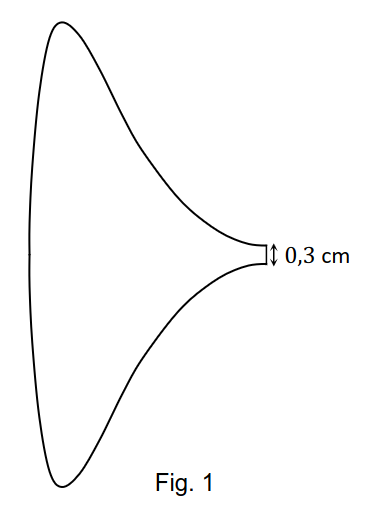
\includegraphics[width=\linewidth]{image_3_exo4.png}
        % \caption{Légende de la première image (optionnel)}
    \end{minipage}
    \hspace{0.5cm}
    \begin{minipage}[c]{0.45\textwidth}
        \centering
        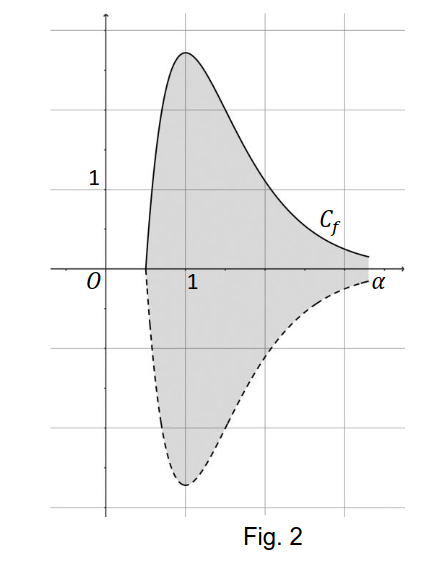
\includegraphics[width=\linewidth]{image_4_exo4.png}
        % \caption{Légende de la deuxième image (optionnel)}
    \end{minipage}
\end{figure}

L'industriel choisit de modéliser le contour de ce logo à l'aide d'une portion de la courbe de la fonction $f$ vue en partie A, et de l'image de cette portion par la symétrie par rapport à l'axe des abscisses, sur un intervalle $[0 ; \alpha]$.
Le nombre $\alpha$ est un réel supérieur à $1$ que l'on déterminera dans cette partie.
L'ensemble est représenté graphiquement dans un repère orthonormé (Fig. 2) d'unité $1\text{ cm}$.

On admet que la fonction $f$ est définie sur l'intervalle $[0 ; +\infty[$ par :
$$f(x) = (2x - 1)\text{e}^{-2x+3}$$

\begin{enumerate}
    \item 
    \begin{enumerate}
        \item[a.] Vérifier que pour tout réel $x$ appartenant à l'intervalle $[0 ; +\infty[$ :
        $$f(x) = \text{e}^2 \times \frac{2x - 1}{\text{e}^{2x-1}}$$
        \item[b.] En déduire la limite de $f$ en $+\infty$.\\
        (On pourra poser $X = 2x - 1$).
    \end{enumerate}
    \item 
    \begin{enumerate}
        \item[a.] Montrer que pour tout $x$ de l'intervalle $[0 ; +\infty[$, $f'(x) = (-4x + 4)\text{e}^{-2x+3}$.
        \item[b.] Construire le tableau complet des variations de la fonction $f$ sur l'intervalle $[0 ; +\infty[$.
    \end{enumerate}
    \item Justifier que la contrainte imposée par le client se traduit par l'égalité $f(\alpha) = 0,15$.\\
    Montrer qu'il existe une unique valeur de $\alpha$ dans l'intervalle $[1 ; +\infty[$ qui permet de vérifier cette égalité. En donner une valeur arrondie au dixième.
\end{enumerate}



\end{document}